% Template for ICIP-2018 paper; to be used with:
%          spconf.sty  - ICASSP/ICIP LaTeX style file, and
%          IEEEbib.bst - IEEE bibliography style file.
% --------------------------------------------------------------------------
\documentclass{article}
\usepackage{spconf,amsmath,graphicx}
\usepackage{epstopdf}
\usepackage{color}
\usepackage{enumerate}
\usepackage{amsmath}
\usepackage{booktabs}


\newcommand{\cxj}[1]{\textcolor[rgb]{1.00,0.00,0.00}{(cxj: #1)}}
\newcommand{\mdf}[1]{\textcolor[rgb]{0.00,0.00,1.00}{#1}}
\newcommand{\drf}[1]{\textcolor[rgb]{0.00,0.50,1.00}{(drf: #1)}}
\newcommand{\vb}[1]{\mathbf{#1}}
\newcommand{\comments}[1]{}
% Example definitions.
% --------------------
\def\x{{\mathbf x}}
\def\L{{\cal L}}

% Title.
% ------
\title{Robust Room Layout Estimation with\\
	Geometric Hints}
%
% Single address.
% ---------------
\name{Authors\thanks{Thanks to XYZ agency for funding.}}
\address{Address}
%
% For example:
% ------------
%\address{School\\
%	Department\\
%	Address}
%
% Two addresses (uncomment and modify for two-address case).
% ----------------------------------------------------------
%\twoauthors
%  {A. Author-one, B. Author-two\sthanks{Thanks to XYZ agency for funding.}}
%	{School A-B\\
%	Department A-B\\
%	Address A-B}
%  {C. Author-three, D. Author-four\sthanks{The fourth author performed the work
%	while at ...}}
%	{School C-D\\
%	Department C-D\\
%	Address C-D}
%
\begin{document}
%\ninept
%
\maketitle
%
\begin{abstract}
We consider the problem of room layout estimation from a single RGB image. Previous methods based on fully convolutional neural networks (FCNs) suffer from heavy occlusion and clutter in indoor scenes. In this paper, we propose to handle these problems with geometric hints and generate more robust layout estimation. Our method consist of three steps: (1) depth and normals are extracted from the RGB image; (2) a multi-channel FCN (MC-FCN) is presented to integrate these geometric hints for semantic surface segmentation; (3) an optimization framework is adopted to refine the layout estimation. The proposed method has proven to be more robust to complex environmental factors. We achieve competitive performance on two commonly used benchmark datasets. 
	
\end{abstract}
%
\begin{keywords}
Layout estimation, scene understanding, geometric hints.
\end{keywords}
%
\section{Introduction}
\label{sec:intro}

The main purpose of room layout estimation is to extract semantic boundaries among walls, ceiling and floor from a single image. It can be realized by obtaining corresponding semantic planes, as shown in Fig. \ref{fig:pipeline}. The task is challenging because of complex environmental factors such as illumination variations, viewpoint shift, object diversity and clutter. Furthermore, distinctive clues like room corners and layout boundaries are often occluded by objects. 

%%
In recent years, massive researches have been carried out on room layout estimation. Conventional methods usually follow a proposing-ranking framework \cite{hedau2009recovering,wang2013discriminative,gupta2010estimating,hedau2010thinking}. Typically, they first generate numbers of proposals through vanishing point detection and ray sampling. Then a ranking step using hand-crafted rules is adopted to select the best hypothesis. Recent methods built on FCNs \cite{long2015fully} or encoder-decoder networks achieve impressive performance \cite{mallya2015learning,ren2016coarse,zhang2017learning,dasgupta2016delay,LeeRoomNet17,zhao2017physics}. Specifically, 
%
Mallya et al.~\cite{mallya2015learning} presented an FCN for learning informative edge maps from images, which were then integrated into the conventional framework as additional features. 
%
Dasgupta et al.~\cite{dasgupta2016delay} used an FCN to learn semantic surface labels including \{Left wall, Front wall, Right wall, Ceiling, Ground\} for each pixel. They obtained a segmentation depended on heat maps from FCN and further refined it with geometric projection constraints.
% 
In a subsequent technique~\cite{ren2016coarse}, Ren \emph{et al}. adopted a multi-task fully convolutional neural network (MFCN) to jointly predict the surface labels and boundaries. Benefit from joint training, the semantic boundaries are more accurate. They also optimized the results later with a refinement framework designed for boundaries.
% 
Zhang \emph{et al}.~\cite{zhang2017learning} proposed an another deconvolution network which has multi-layer deconvolution and a receptive field as large as the entire image compared to FCN. As a result, they attained highly reliable edge maps. 
%
An end-to-end approach for room layout estimation was explored by Lee \emph{et al}.~\cite{LeeRoomNet17}. They employed an encoder-decoder network to delineate the room layout structure using 2D keypoints.
%
Zhao \emph{et al}. \cite{zhao2017physics} introduced a semantic transfer FCN to extract reliable edge features. They first trained an FCN for 37-class semantic segmentation and then bridged the gap to 4-class edge labels by adding a fully connected layer. A physics inspired inference scheme was designed for optimization.


Different from previous FCN based methods, we propose to improve the performance of room layout estimation from another perspective. We consider global geometric information as important as the texture in room layout estimation. To implicitly employ the geometric hint, depth and normals are estimated from the original image and fused into an multi-channel FCN. We use the same formulation of layout in \cite{dasgupta2016delay} and combine their optimization step with a proposing-ranking framework to attain precise layout. Experimental results demonstrate that our method is robust and effective for layout estimation even facing clutter and occlusion.

\comments{
In this paper, we propose to enhance the FCN's ability for room layout estimation by fully utilizing the geometric information of the scene. Our pipeline is shown in Fig.~\ref{fig:pipeline}. First, we estimate depth and normal maps from a single image using network in \cite{eigen2015predicting}. Then we integrate these geometric hint to train a multi-channel FCN for semantic surface segmentation. At last, an extended post-processing algorithm based on \cite{dasgupta2016delay} is applied to generally refine the estimation results. We evaluate our method on two popular benchmark dataset. Experimental results demonstrate that our method is robust and effective for layout estimation even facing clutter and occlusion.
}






\section{Our Method}
\label{sec:Meth}


\subsection{System Overview}
\label{subsection:overview}

\begin{figure}[!ht]
	\centering
	\includegraphics[width=3.4in]{figure/pipeline.eps}
	\caption{An overview of our layout estimation algorithm pipeline. First we adopt a multi-scale CNN achitecture \cite{eigen2015predicting} to extract geometric information from RGB images, including depth and normals. Then we combine all the abovementioned information into a multi-channel FCN , which helps to accurately estimate the layout. An optimization framwork based on perspective projection restriction is then used to generate final precise layout estimates.}
	\label{fig:pipeline}
\end{figure}

Under the Manhattan world assumption, a room layout can be represented as a cube having at most five surfaces (Three walls, Ceiling, Ground) visible in the image. 
%
Given an RGB image $\vb{I}$ with arbitrary size, our algorithm generates a room layout $\vb{L}$ consisting of a surface label for each pixel $L_{ij}\in $ $\{$Left, Front, Right, Ceiling, Ground$\}$. 
Fig. \ref{fig:pipeline} shows our algorithm pipeline. 
%%step 1
Different from \cite{dasgupta2016delay}, we first estimate depth map $D_{I}$ and normal map $N_{I}$ from the input color image to generate geometric hints using a multi-scale convolutional architecture~\cite{eigen2015predicting}, as described in Sec.~\ref{sec:depth_normal}.
%step 2
After that, to integrate information from the original RGB image together with the geometric hints, a fully convolutional network with multi-channel input is applied to predict five probability maps, each of which describes the belief for a specific layout surface, see details in Sec.~\ref{sec:surfacelabel}.
%step 3: optimization
While we can easily get access to the final layout estimation by just choose the label with highest score across the five probability maps for each pixel. 
The estimated $\vb{L}$ always have wavy boundaries and multiple disjoint connected domains due to the characteristics of neural network. To handle these problems and obtain more clear layout estimation with geometric constraints, an optimization step is adopted in Sec.~\ref{sec:optimization}.  
 

\comments{
The coarse layout estimation about semantic layout surfaces for a single RGB image, are predicted by fully convolutional neural network with geometric information emmbeded, including depth and normal information. These geometric information are estimated from source RGB image by a multi-scale convolutional architecture\cite{eigen2015predicting}. This will be decribied in Sec. \ref{subsection:CNN}. Then based on optimization framwork proposed in \cite{dasgupta2016delay}, which mainly uses perspective projection constraints, we can obtain final precise layout estimation results.
%
}


\subsection{Geometric Hints Extraction}
\label{sec:depth_normal}

We use the multi-scale convolutional network proposed in \cite{eigen2015predicting} to estimate the depth and normal map from a single RGB image, as shown in Figure~\ref{fig:depthandnormal}. Note that we do not finetune their models with our data as we do not have the depth and normals of our dataset, however, the model seems to generalize well in our case. From the global perspective, the depth and normal maps we obtained capture the overall spatial relationships between semantic surfaces. Quantitive evaluation for depth and normals extraction can be refered to in ~\cite{eigen2015predicting}.
%

\begin{figure}
	\centering
	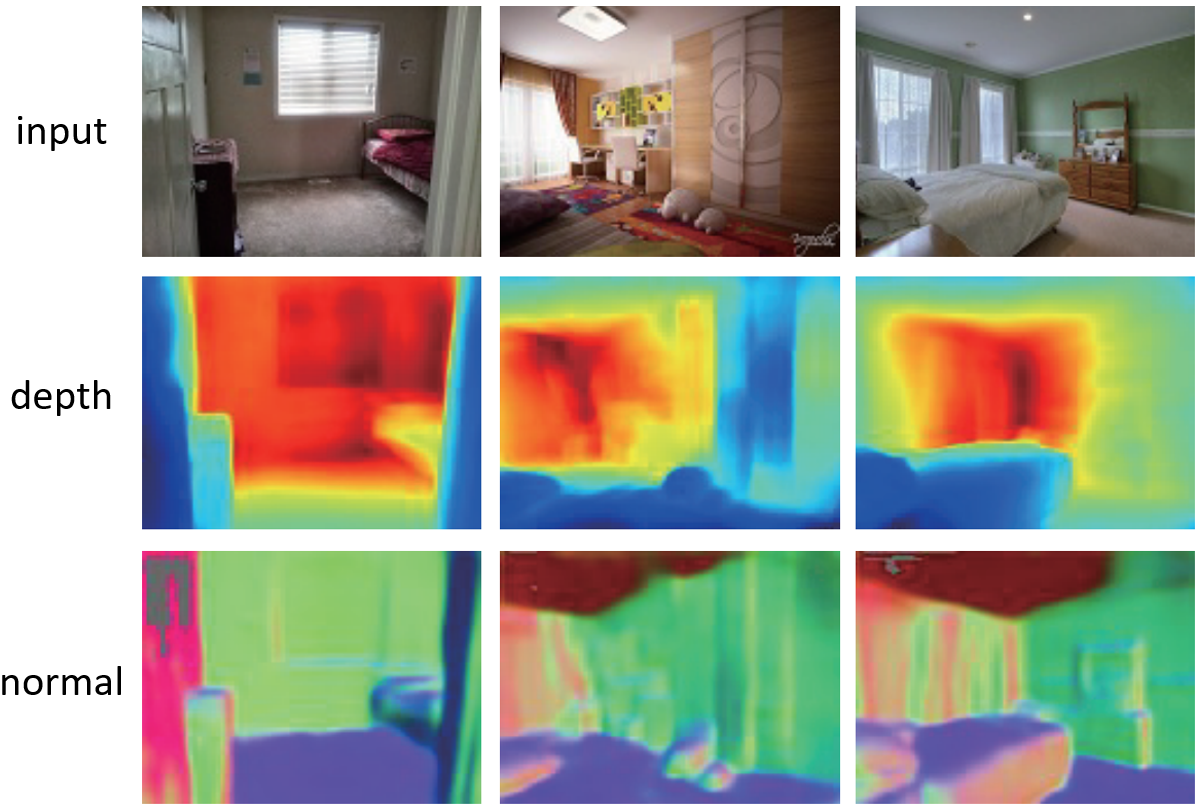
\includegraphics[width=\columnwidth]{figure/geometricinfo1.png}
	\caption{Estimation of depth and normal from a single RGB image using the multi-task FCN in \cite{eigen2015predicting}.}
	\label{fig:depthandnormal}
\end{figure}

We notice in practice that the depth maps and surface maps estimated from single RGB images are not precise in local details. And the The output resolution of the depth maps and normal maps are limited to half of the input. However, the valuable 3D information they provide is much helpful for high-level structure estimation, especially in cluttered scenes.  
%
Normals can serve as clues tending to merge big planes together, with interference factors like clutter, textures and illumination eliminated to varying degrees. 
%
These mid-level geometric information can be used to adapt and improve performance for layout estimation compared to using RGB only. 

The depth maps are color coded in \cite{eigen2015predicting} for distinction. In order to reduce the redundant information and to ensure the essence of depth, We modify their rendering section to obtain depth maps with single channel while preserving the optimization part.

\subsection{Surface Label Prediction Using MC-FCN}
\label{sec:surfacelabel}
%
In previous work, fully convolutional neural network(FCNN) or multi-task fully convolutional neural network~(MFCNN) are used to predict coarse semantic layout surfaces or layout edges \cite{dasgupta2016delay,ren2016coarse,zhao2017physics,zhang2017learning}. 
%
However, due to much clutter, complex textures and illumination variations, semantic surfaces like walls are visually separated in to pieces, making whole surfaces difficult to aggregate together. 
%
Fig.~\ref{fig:fcn-comparison}(b) shows some bad semantic surface predicting results from a widely used FCNN architecture in previous methods \cite{dasgupta2016delay,ren2016coarse}. 
The comparison between the predicted results and the ground truth reveals that due to the complex environmental factors of indoor scenes, layout results estimated from FCNN are not very reliable sometimes. 
When the occlusion happens to be at the boundaries of semantic planes, such critical clues are partially or entirely excluded, and thus we can not tell location of each plane precisely. 
Moreover, an entire plane may be predicted separately into pieces due to clutter lay in the plane.


\begin{figure}
	\centering
	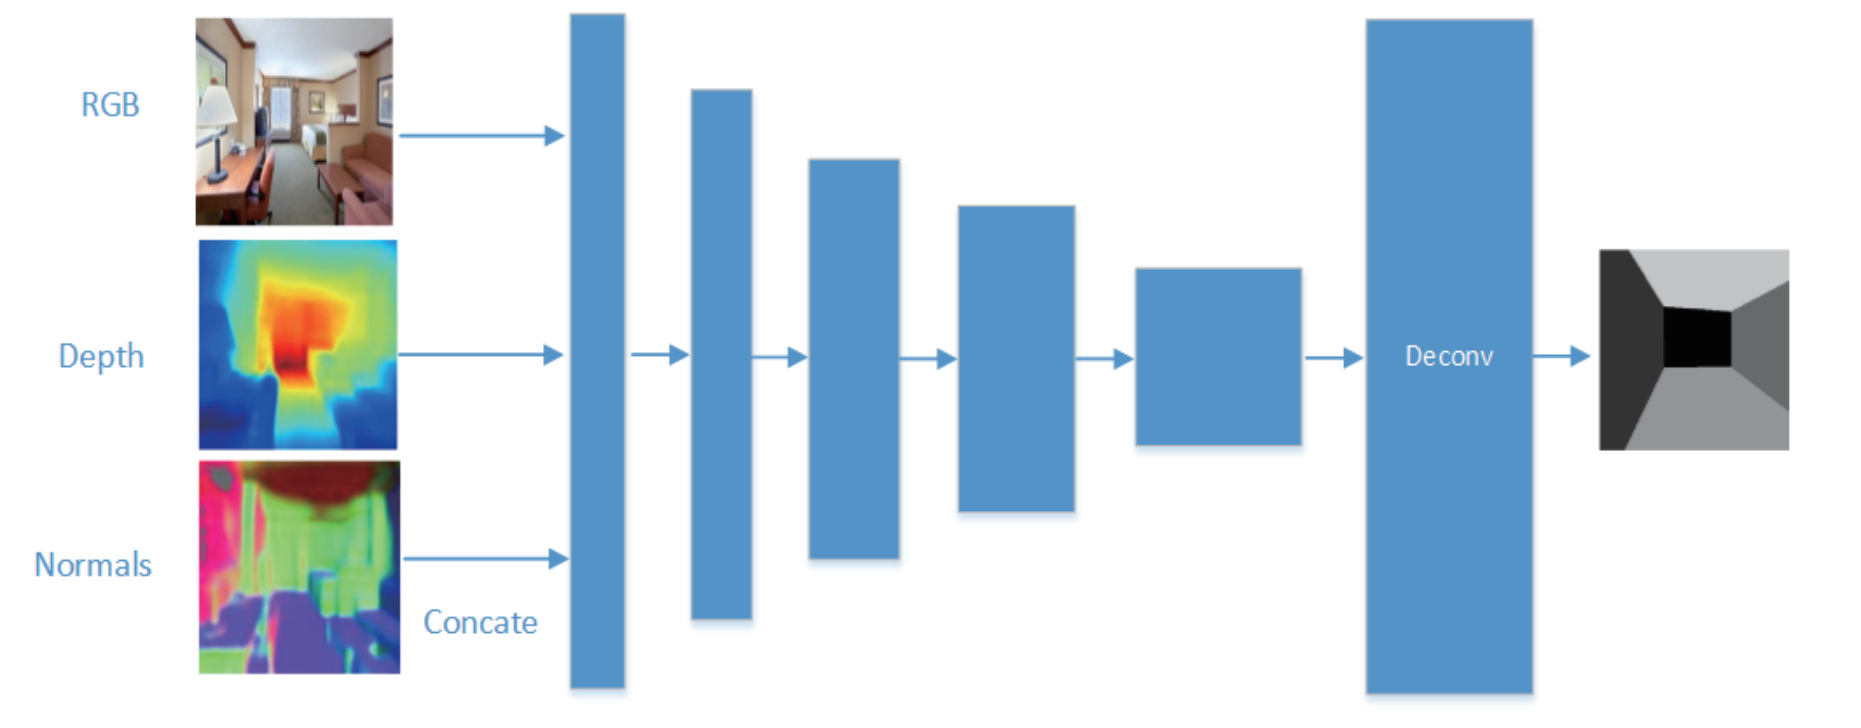
\includegraphics[width=\columnwidth]{figure/fcn-multi-channel.png}
	\caption{Illustration of the multi-channel network architecture build on \cite{chen2016deeplab}. We combine the RGB image, depth and normal together as input to the ResNet101 based FCN for semantic surface learning. }
	\label{fig:fcn-multi-channel}
\end{figure}


\textbf{Network Architecture}
To alleviate the problems caused by complex environmental factors, we fuse the geometric hints with original texture information and train a multi-channel input FCN. As Fig.~\ref{fig:fcn-multi-channel} shows, We build this multi-channel FCN on the famous architecture ResNet-101 \cite{he2016deep} modified by \cite{chen2016deeplab}. The estimated depth and normal maps are treated as additional channels associated with the input RGB images. 

\textbf{Training}
We simply concatenate different types of data to a seven-channels input(3 channels from RGB, 1 channel from depths and 3 channels from normals) which is then fed into our network. The FCN model we used for initialization from \cite{chen2016deeplab} is pretrained on MS-COCO dataset. We randomly initialize the weights for the first convolution layer to adapt to our input format and replace the weights for classifier layer with randomly initialized 5-way classifier layer. Then we specifically finetune our multi-channel FCN for semantic surface segmentation. We have also tried multi-task learning by adding a new branch for learning boundaries between surfaces as \cite{ren2016coarse, mallya2015learning} do. But the joint training doesn't help to improve the performance of both task in our case. This may indicate that our geometric hints have already integrated the additional information which should be learned through joint training.

The output of our multi-channel FCN is a $w\times h \times 5$ multidimensional array $\vb{T}$, where w and h stand for the width and length of the input rgb image. Each of the 5 slices can be viewd as a probability map for the corresponding surface label. Some visualized results compared with FCN without geometric hints as additional input are shown in Fig.~\ref{fig:fcn-comparison}. We utilize the probability array $\vb{T}$ as the basis for our scoring function. Then an optimization step based on this score function is applied to obtain precise layout estimation.


\begin{figure}[!ht]
	\centering 
	\textsc{\includegraphics[width=3.4in]{figure/fcn.eps}}
	\caption{Layout estimation results using different architectures. Row from top to bottom: (a) the input RGB image. (b) Surface predictions using the FCNN architecture used in \cite{dasgupta2016delay,ren2016coarse}. (c) our MC-FCN. (d) The ground truth. Our method generate much more clear edges, less holes.}
	\label{fig:fcn-comparison}
\end{figure}


\subsection{Layout Generation}
\label{sec:optimization}
We adopt a popular model that several researchers ~\cite{hedau2009recovering, wang2013discriminative, dasgupta2016delay, ren2016coarse} have used to parameterize indoor layout based on the Manhattan world assumption. 
Indoor scene layout is modeled as the projection of a cuboid which can be defined by 

\begin{equation}
	\label{eq:Layout}
	L = (l1, l2, l3, l4, v)
\end{equation}

where $l_{i}$ stands for $i^{th}$ line and $v$ stands for the specific vanishing point. The whole scene is equivalent to be labeled with five semantic surfaces, coresponding to \{Left, Front, Right, Ceiling, Ground\}, as described in Fig. \ref{fig:2.model}. Based on Eq. (\ref{eq:Layout}), each surface can be reconstructed with extension lines between vanishing point $v$ and Intersection point $p_i$ among $l_{i}$. ie $ve_i$ . Due to the uncertainty of camera pose, five surfaces are not always visible. Examples with different topologies are given in Fig. \ref{fig:different-layout-type}.


To obtain the optimized box layout $\vb{L}$, \cite{dasgupta2016delay} has propose a refinement algorithm. They first generate an initial $\vb{\hat{L}}$ by pick the label with the highest score across five channels of $\vb{T}$. Then a preprocessing step is used to address spurious regions and multiple disjoint components in $\vb{\hat{L}}$. Finally, an iterative optimization method is employed to acquire the refined $\vb{L}$. However, the initial $\vb{\hat{L}}$ generated from $\vb{T}$ are sometimes too ambiguous due to the characteristics of neural network. The preprocessing step can't adapt to all the bad situations well, especially when the ambiguous walls are close in size. 


To make the optimization method more general and efficient, we simplify the refinement algorithm in \cite{dasgupta2016delay} by replace the first two step with a proposing-ranking framework. Our proposing-ranking framework directly generate an initial $\vb{\hat{L}}$ that consistent with the definition in Eq.~\ref{eq:Layout}. This kind of $\vb{\hat{L}}$ are much robust to ambiguous cases and easier for the optimization step to find the refined layout.

The proposing-ranking framework is implemented by extracting enough proposals using the approach in \cite{hedau2009recovering} and a score function based on $\vb{T}$. We sample 30 rays per vanishing point to acquire enough proposals. Then we extend the modified score function in \cite{dasgupta2016delay} for special cases to adapt to all images. Given a specific label, We simply sum up the probability across 5 channels of $\vb{T}$ seperately in the same region and choose the maximum as the score for this specific label. This policy is applied just among three walls which mainly cause the ambiguity. The same extended score function is adopted in optimization step. Our postprocessing framework generalize well to ambiguous cases.

\comments{
\textbf{Preprocessing} 
Although we have more robust surface prediction result from our FCN-MC. Problems like spurious regions and multiple disjoint components are still a bit disturbing. To address these problems we simplify the preprocessing step in ~\cite{dasgupta2016delay} for efficiency. First, we address the multiple disjoint components (which means the connection domain for each label is not unique) by remove all but the largest connected domain for each label. Then we fill the holes created by this pruning with labels around them by using k-nn. After that we apply some simple contraints based on common sense to handle spurious regions.}

\begin{figure}
	\centering
	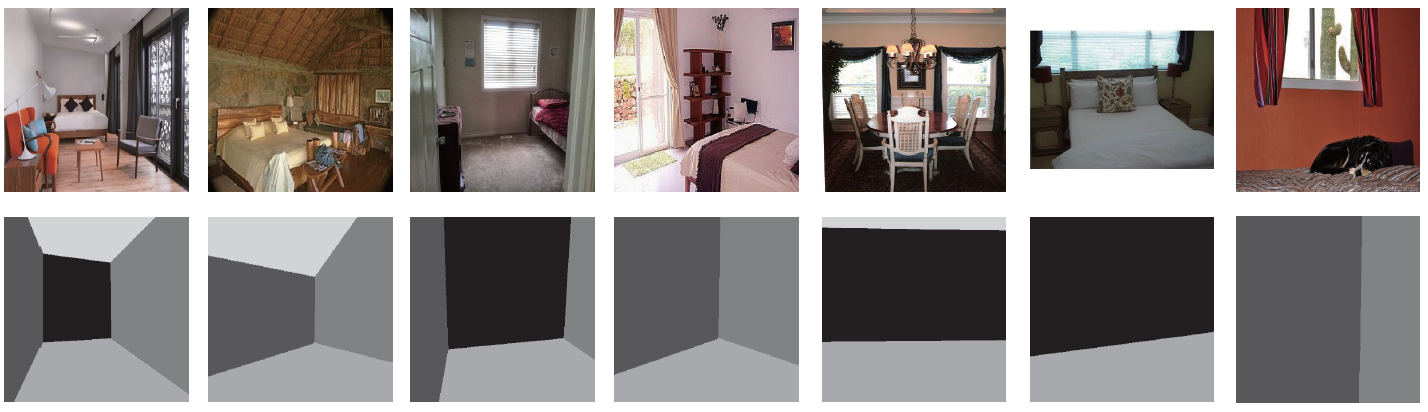
\includegraphics[width=\columnwidth]{figure/different-layout-type.png}
	\caption{Different layout type due to variation in camera pose. \drf{I'm not sure whether this situation should be discussed, so the caption is brief.} }
	\label{fig:different-layout-type}
\end{figure}
\section{RESULTS}
\label{sec:Res}

We prove the validity of the geometric hints in semantic surface segmentation and evaluate our method on two widely used dataset: Hedau's dataset \cite{hedau2009recovering} and LSUN dataset \cite{zhang2015large}. 

\subsection{Analysis of Geometric Hints}
\label{sec:ablation}
To explore the benefits of geometric hints for semantic surface segmentation, we train FCNs with or without geometric hints as additional input. Their performance are evaluated on LSUN validation set using pixel error of $\vb{\hat{L}}$, see Table~\ref{table:ablation}. To make fair comparisons with \cite{ren2016coarse, dasgupta2016delay}, both of which are built on VGG16, we train an MC-FCN based on VGG16 too. For \cite{ren2016coarse}, we directly apply their trained model to generate $\vb{\hat{L}}$. And for \cite{dasgupta2016delay}, we train an FCN having the same architecture in \cite{dasgupta2016delay}. As revealed by Table~\ref{table:ablation}, with the help of geometric hints, our MC-FCN obtain lower pixel error of $\vb{\hat{L}}$. We further improve the performance by employing a ResNet101 based FCN. Qualitative results are demonstrated in Fig.~\ref{fig:fcn-comparison}. (a)-(e) show typical good examples. Intuitively, the geometric hints help remove the spurious regions caused by clutter and generate more accurate semantic surface segmentation. (f) depicts a generally bad case that FCNs tend to be cheated by large truncated wall-like object surface, e.g., the bed looks like the floor. (g) is an another kind of bad case led by clutter while our MC-FCN seems to produce relatively clear results.  

\begin{figure}[!ht]
	\centering 
	\textsc{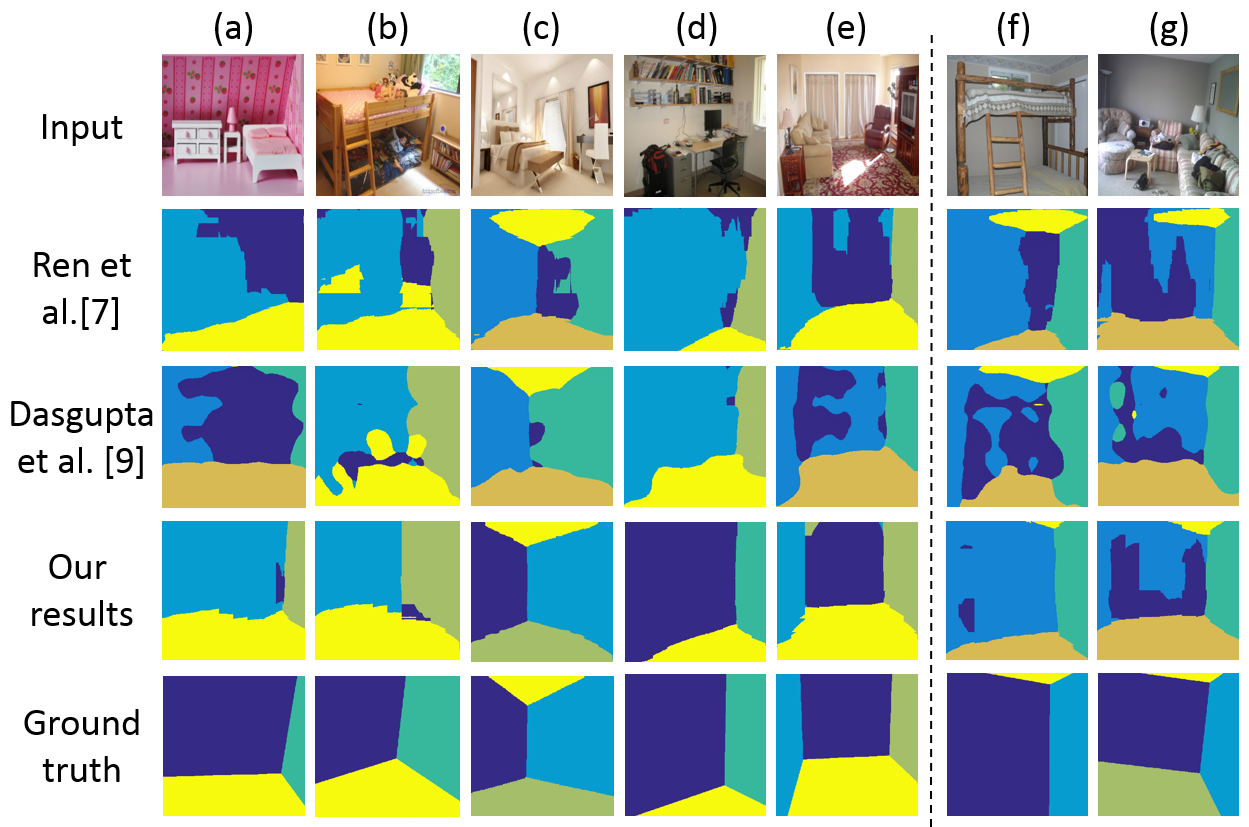
\includegraphics[width=8.5cm]{figure/compare1.png}}
	\caption{Surface segmentation results using different architectures. All the networks are built on VGG16 architecture. Our MC-FCN with geometric hints generates more robust segmentation facing complex environmental factors.}
	\label{fig:fcn-comparison}
\end{figure}

\begin{table}
	\centering
	\begin{tabular}{lc}
		\toprule
		Network & $\epsilon_{pixel}$ (\%)\\
		\midrule
		Ren et al.~\cite{ren2016coarse} & 21.54 \\
		Dasgupta et al.~\cite{dasgupta2016delay} & 15.86 \\  
		\midrule
		MC-FCN (VGG16)  & 14.05 \\
		MC-FCN (ResNet101) & 12.41 \\
		\bottomrule
	\end{tabular}
	\caption{Pixel error of semantic surface segmentation by different FCNs. By utilizing geometric hints, our proposed MC-FCN acquire more accurate segmentation. }	
	\label{table:ablation}
\end{table}

\subsection{LSUN Results}
\label{sec:LSUN}
We train our multi-channel FCN on the relabeled LSUN dataset released by \cite{ren2016coarse}. The dataset consists of 4000 training, 394 validation, and 1000 testing images. We extract geometric hints from original images and resize all the images, depth and normal maps to $321\times321$ using bicubic interpolation. Then these three types of data are integrated to train the ResNet101 based multi-channel FCN. We evaluate our results using the official toolkit which provides two standard metrics: pixelwise error and corner error. The pixelwise error is computed by counting the percentage of pixels that are mismatched. (The Hungarian algorithm is applied to address the labeling ambiguity problem) The corner error is computed by calculating the Euclidean distance between predicted corners and corresponding ground truth corners.

Our performance on LSUN test set compared with other methods is shown in Table~\ref{table:comparison-lsun}. Qualitative results are displayed in Fig.~\ref{fig:qualitative}. Our approach outperforms conventional methods \cite{hedau2009recovering} and most neural network based methods  \cite{mallya2015learning,zhang2017learning,dasgupta2016delay,ren2016coarse,LeeRoomNet17}. 
%
Besides, when training the FCN, Zhao et al.~\cite{zhao2017physics} formulate the room layout using boundaries among semantic surfaces, while we formulate the room layout using the five semantic surfaces as \cite{dasgupta2016delay} do. These two representation may have different application prospects in the future. For example, when a home robot wants to locate itself while moving, the semantic boundaries are not always available. Our method may also be an inspiration for other surface detection problems.

\comments{
This kind of boundary representation has a intrinsic problem of unbalanced training data where most of the area is background. This may be the reason for the training problem, as claimed in \cite{zhao2017physics,mallya2015learning}. They both have to pretrain their model on an indoor scene dataset to make the training stable. While we formulate the room layout using the five semantic surfaces as \cite{dasgupta2016delay} do, our representation does not have this limitation. We pretrain our MC-FCN on both indoor scene dataset (SUNRGBD) and non-indoor scene dataset (PASCAL) separately. Both settings lead to stable training and competitive performance, as shown in \ref{table:comparison-lsun}. The model pretrained on SUNRGBD obtains a better result which should benefit from external indoor scene data in SUNRGBD. }


\comments{
This boundary representation and its variants are adopted in \cite{zhang2017learning,ren2016coarse}, while we formulate the room layout using the five semantic surfaces as \cite{dasgupta2016delay} do. 
%
Which formulation is better for room layout estimation remains an open question, especially when the room can not be exactly modeled as a cube due to special architectural structures such as slope roof, pillar and condole top. Boundary representation may be less robust to these situations and LSUN dataset contains few of these cases. Moreover, the two representation may work togehter to improve both performance in a joint training way, which is possible claimed by \cite{mallya2015learning,ren2016coarse}.}


\begin{figure}[!ht]
	\centering
	\textsc{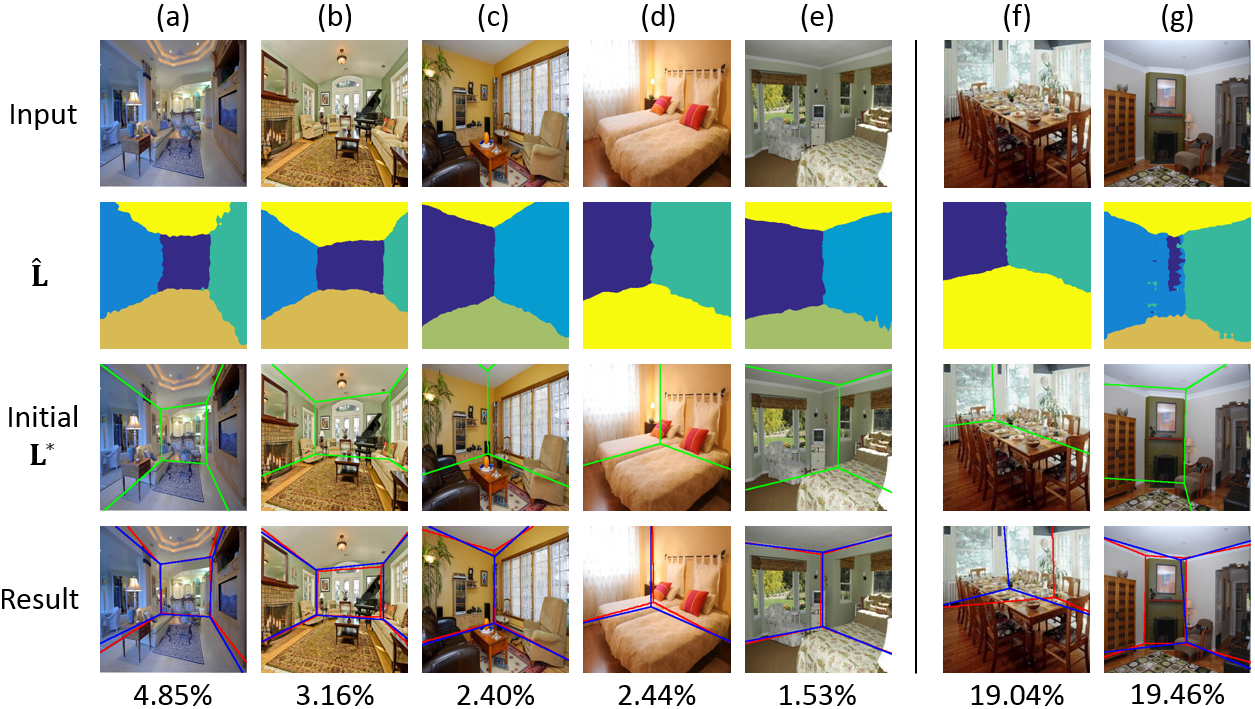
\includegraphics[width=8.5cm]{figure/qualitive.png}}
	\caption{Qualitative results of our methods on LSUN validation set. (a)-(e) depict precise results. (f)(g) show failure cases misled by $\vb{\hat{L}}$. }
	\label{fig:qualitative}
\end{figure}

\begin{table}
	\centering 
	\begin{tabular}{lcc}
		\toprule
		Method & $\epsilon_{corner}$ (\%) & $\epsilon_{pixel}$ (\%) \\
		\midrule
		Hedau et al.~\cite{hedau2009recovering} & 15.48 & 24.23 \\
		Mallya et al.~\cite{mallya2015learning} & 11.02 & 16.71 \\
		Zhang et al.~\cite{zhang2017learning} & 8.70 & 12.49 \\
		Dasgupta et al.~\cite{dasgupta2016delay} & 8.20 & 10.63 \\
		Ren et al.~\cite{ren2016coarse} & 7.95 & 9.31 \\
		Lee et al.~\cite{LeeRoomNet17} & 6.30 & 9.86 \\
		Zhao et al.~\cite{zhao2017physics} & 3.84 & 5.29 \\
		\midrule
		Proposed MC-FCN & 6.26 & 8.61 \\
		\bottomrule
	\end{tabular}
	\caption{Performance on the LSUN~\cite{zhang2015large} dataset}	
	\label{table:comparison-lsun}
\end{table}

\subsection{Hedau Results}
\label{sec:Hedau}
We also conduct experiment on a relatively smaller dataset published by \cite{hedau2009recovering}, which consists of 209 training images and 104 testing images. We follow the experimental setup in \cite{LeeRoomNet17} and directly predict the semantic surface on Hedau's test set using the model trained on LSUN. Pixel error is adopted to evaluate the final results, see Table~\ref{table:comparison-hedau}. Our performance is better than \cite{mallya2015learning,zhang2017learning,ren2016coarse}, all of which have trained their model on Hedau's training set. This indicates that our model has a good generalization ability. We achieve the performance close to state-of-the-art on this dataset.

\begin{table}
	\centering 
	\begin{tabular}{lc}
		\toprule
		Method & $\epsilon_{pixel}$ (\%) \\
		\midrule
		Hedau et al.~\cite{hedau2009recovering} & 21.20 \\
		Mallya et al.~\cite{mallya2015learning} & 12.83 \\
		Zhang et al.~\cite{zhang2017learning} & 12.70 \\
		Dasgupta et al.~\cite{dasgupta2016delay} & 9.73 \\
		Ren et al.~\cite{ren2016coarse} & 8.67 \\
		Lee et al.~\cite{LeeRoomNet17} & 8.36 \\
		Zhao et al.~\cite{zhao2017physics} & 6.60 \\
		\midrule
		Proposed MC-FCN & 6.07 / 7.90 \\
		\bottomrule
	\end{tabular}
	\caption{Performance on the Hedau's~\cite{hedau2009recovering} dataset \drf{6.07 using the metric in \cite{LeeRoomNet17}, 7.90 using the metric in \cite{zhao2017physics}}}
	\label{table:comparison-hedau}
\end{table}




\section{CONCLUSION}
\label{sec:Con}

In this paper, we propose to fully utilize the geometric information from an RGB image for room layout estimation. We estimate the depth and normal maps from the input color image and then combine them together to train a multi-channel FCN. We demonstrate how these geometric hints improve the performance of semantic surface segmentation. Then we incorporate a proposing-ranking policy to generally optimize the room layout. Benefit from these techniques, our method is robust to complex environmental factors in indoor scenes.


% Below is an example of how to insert images. Delete the ``\vspace'' line,
% uncomment the preceding line ``\centerline...'' and replace ``imageX.ps''
% with a suitable PostScript file name.
% -------------------------------------------------------------------------
\comments{
\begin{figure}[htb]

\begin{minipage}[b]{1.0\linewidth}
  \centering
  \centerline{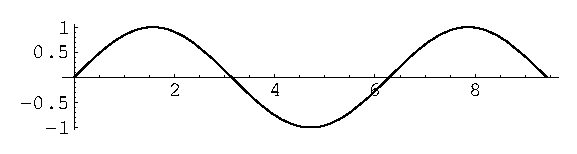
\includegraphics[width=8.5cm]{figure/image1}}
%  \vspace{2.0cm}
  \centerline{(a) Result 1}\medskip
\end{minipage}
%
\begin{minipage}[b]{.48\linewidth}
  \centering
  \centerline{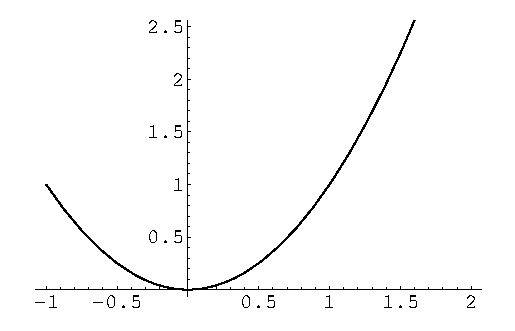
\includegraphics[width=4.0cm]{figure/image3}}
%  \vspace{1.5cm}
  \centerline{(b) Results 3}\medskip
\end{minipage}
\hfill
\begin{minipage}[b]{0.48\linewidth}
  \centering
  \centerline{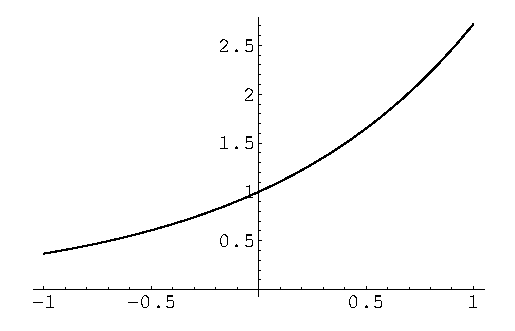
\includegraphics[width=4.0cm]{figure/image4}}
%  \vspace{1.5cm}
  \centerline{(c) Result 4}\medskip
\end{minipage}
%
\caption{Example of placing a figure with experimental results.}
\label{fig:res}
%
\end{figure}
}

% To start a new column (but not a new page) and help balance the last-page
% column length use \vfill\pagebreak.
% -------------------------------------------------------------------------
%\vfill
%\pagebreak
\comments{
\section{COPYRIGHT FORMS}
\label{sec:copyright}

You must include your fully completed, signed IEEE copyright release form when
form when you submit your paper. We {\bf must} have this form before your paper
can be published in the proceedings.
}

% References should be produced using the bibtex program from suitable
% BiBTeX files (here: strings, refs, manuals). The IEEEbib.bst bibliography
% style file from IEEE produces unsorted bibliography list.
% -------------------------------------------------------------------------
\bibliographystyle{IEEEbib}
\bibliography{refs}

\end{document}
